\begin{frame}[c]
    \frametitle{基于像素化介质超表面的分子条形码成像}
    \begin{columns}
        \begin{column}{.7\textwidth}
            \begin{itemize}
                \item Tittl, A.;  Leitis, A.;  Liu, M.;  Yesilkoy, F.;  Choi, D.-Y.;  Neshev, D. N.;  Kivshar, Y. S.; Altug, H., Imaging-based molecular barcoding with \textcolor{purple}{pixelated dielectric} \textcolor{red}{metasurfaces}. Science 2018, 360 (6393), 1105-1109.
                \item \textcolor{blue}{原理:}由吸附蛋白质前后的反射光谱变化分析蛋白质成分。
                \item \textcolor{blue}{创新点:}无需频率扫描或移动机械部件即可解析吸收指纹。
                \item \textcolor{blue}{意义:}为开发灵敏且多功能的微型中红外光谱设备铺平了道路。
                \item ?还没整明白超平面(metasurface)是什么
            \end{itemize}
        \end{column}
        \begin{column}{.3\textwidth}
            \begin{figure}[H] %H为当前位置,!htb为忽略美学标准,htbp为浮动图形
                \centering %图片居中
                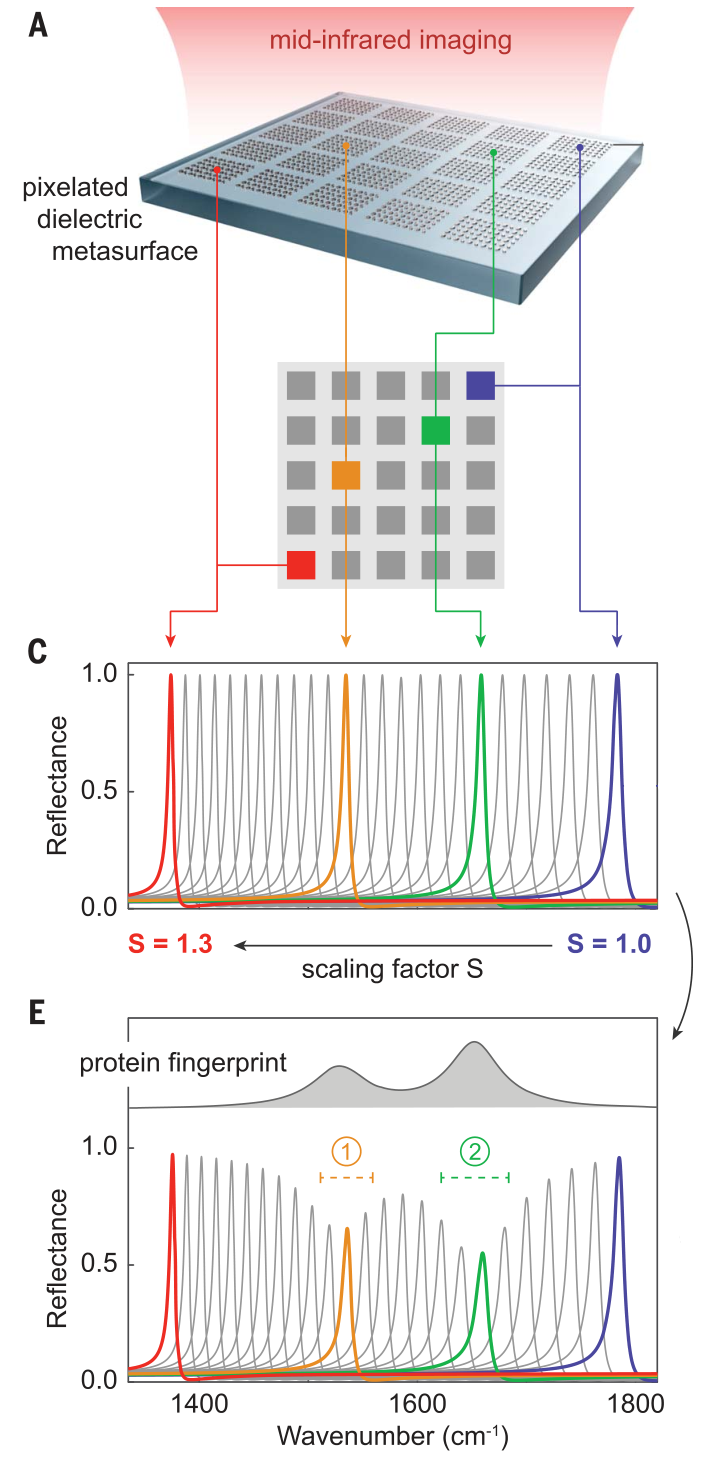
\includegraphics[width=.9\textwidth]{figures/Imaging-based molecular barcoding with pixelated dielectric metasurfaces_1.png} %插入图片,[]中设置图片大小,{}中是图片文件名
            \end{figure}
        \end{column}
    \end{columns}
    \begin{figure}[H] %H为当前位置,!htb为忽略美学标准,htbp为浮动图形
        \centering %图片居中
        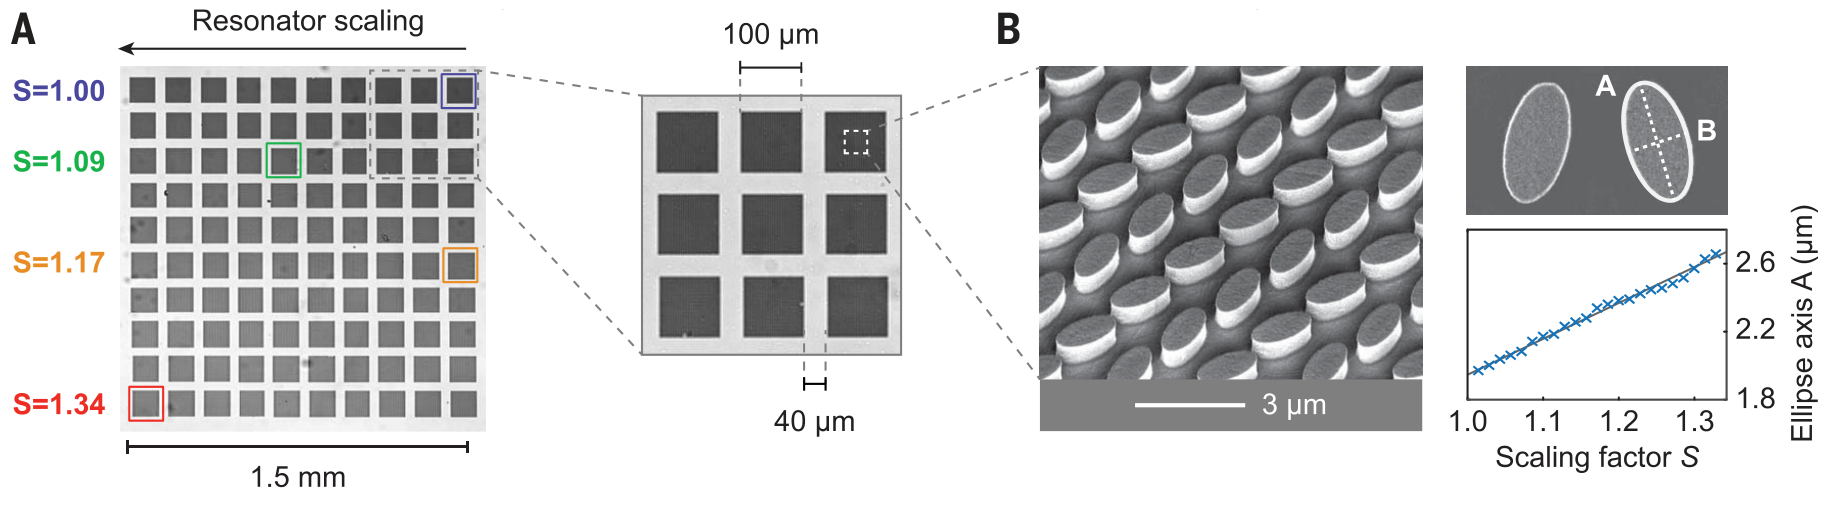
\includegraphics[width=1.\textwidth]{figures/Imaging-based molecular barcoding with pixelated dielectric metasurfaces_2.png} %插入图片,[]中设置图片大小,{}中是图片文件名
    \end{figure}
\end{frame}